\section{RBD Model}
\label{sec:RBDmodel}

This model is designed to read from file the structure of the reliability block diagram (RBD) and import such Boolean logic structure as a RAVEN model.
The RBD must be specified in a specific format. As an example, the RBD of Fig.~\ref{fig:RBD} is translated in the RAVEN format as shown below:

\begin{lstlisting}[style=XML,morekeywords={anAttribute},caption=RBD input file., label=lst:RBDmodel]
<Graph name="testGraph">
  <node name="CST">
    <childs>1</childs>
  </node>
  <node name="1">
    <childs>2,3,4</childs>
  </node>
  <node name="2">
    <childs>5</childs>
  </node>
  <node name="3">
    <childs>5</childs>
  </node>
  <node name="4">
    <childs>5</childs>
  </node>
  <node name="5">
    <childs>6,7,8</childs>
  </node>
  <node name="6">
    <childs>SG1</childs>
  </node>
  <node name="7">
    <childs>SG2</childs>
  </node>
  <node name="8">
    <childs>SG3</childs>
  </node>
  <node name="SG1">
  </node>
  <node name="SG2">
  </node>
  <node name="SG3">
  </node>
</Graph>
\end{lstlisting}

\begin{figure}
    \centering
    \centerline{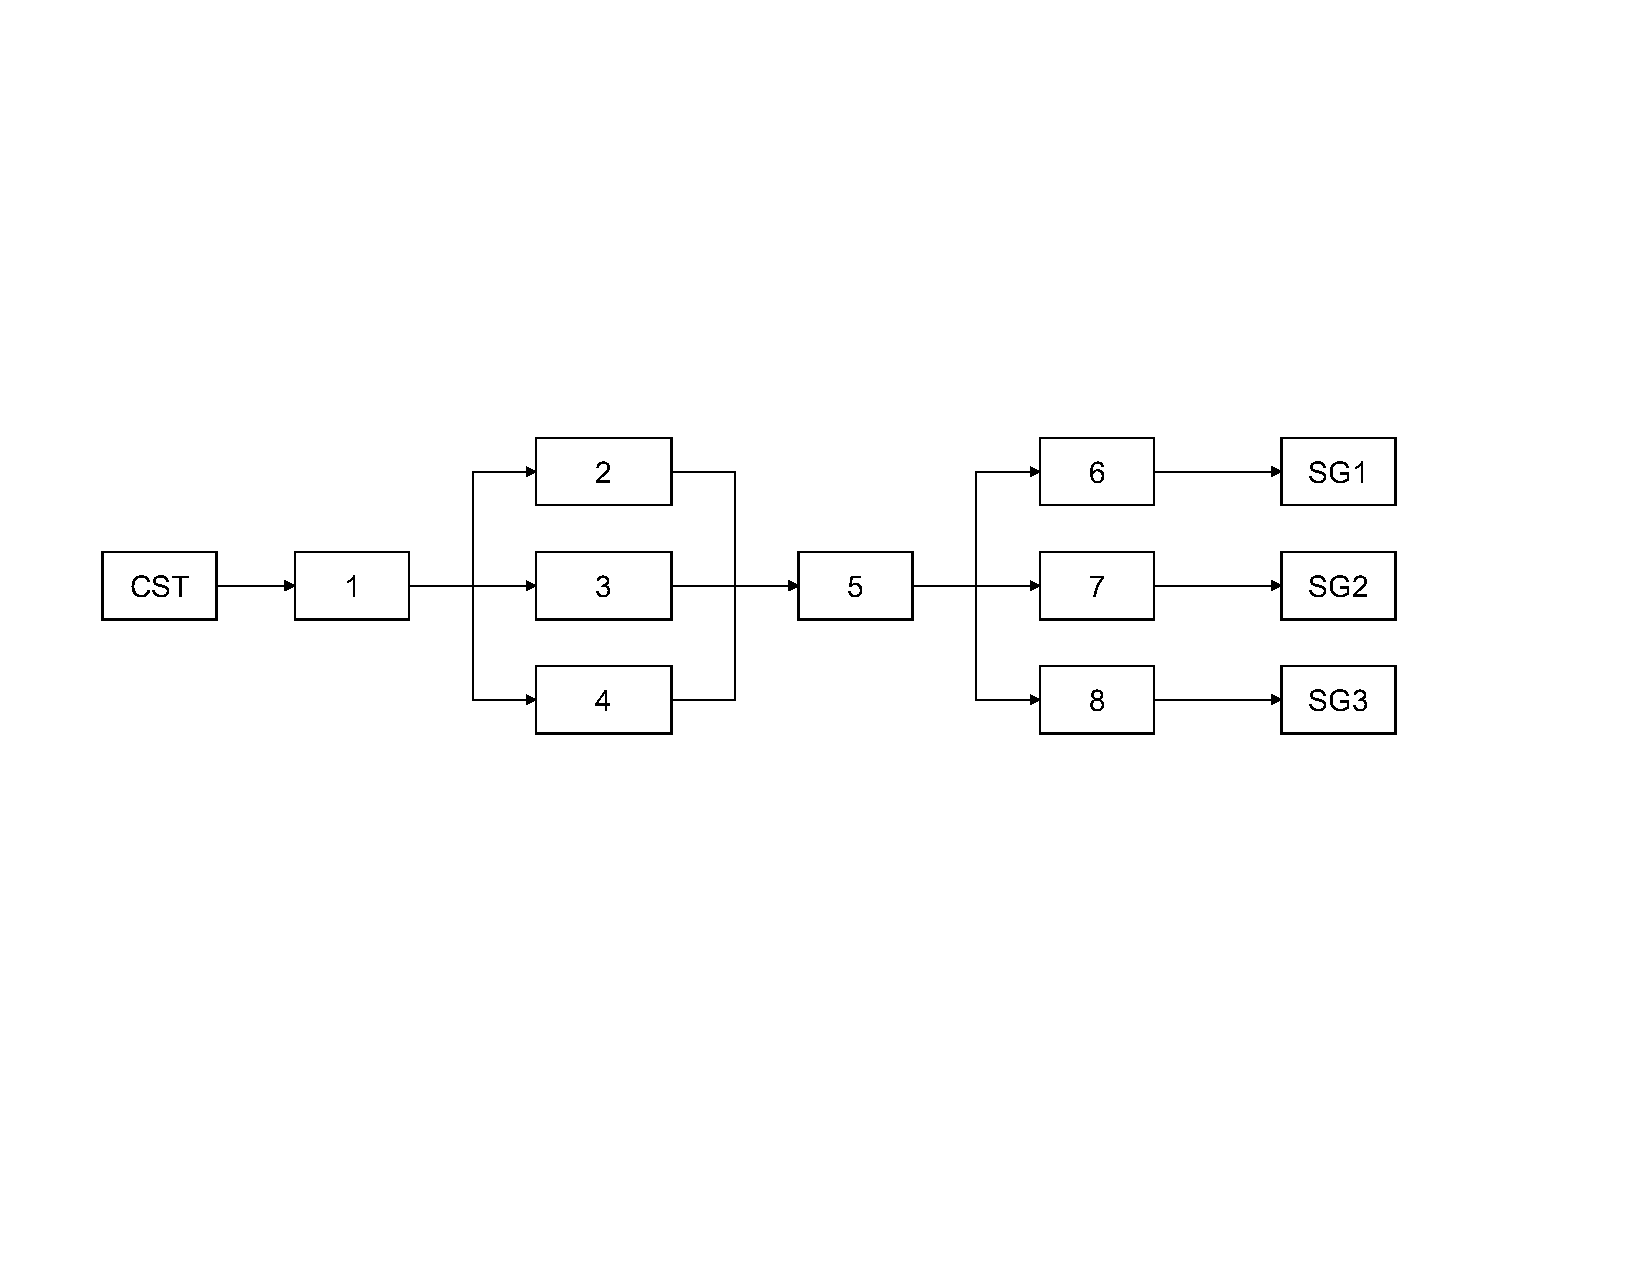
\includegraphics[scale=0.5]{RBD.pdf}}
    \caption{Example of RBD.}
    \label{fig:RBD}
\end{figure}

The FT of RBD illustrated in Fig.~\ref{fig:RBD} and defined in Listing~\ref{lst:RBDmodel} can be defined in the RAVEN input file as follows:

\begin{lstlisting}[style=XML,morekeywords={anAttribute},caption=RBD model input example., label=lst:RBD_InputExample]
  <Models>
    ...
    <ExternalModel name="graph" subType="GraphModel">
      <variables>
        status2,status3,status4,status5,
        statusSG1,statusSG2,statusSG3
      </variables>
      <modelFile>graphTest</modelFile>
      <nodesIN>CST</nodesIN>
      <nodesOUT>SG1,SG2,SG3</nodesOUT>
      <map var="status2">2</map>
      <map var="status3">3</map>
      <map var="status4">4</map>
      <map var="status5">5</map>
      <map var="statusSG1">SG1</map>
      <map var="statusSG2">SG2</map>
      <map var="statusSG3">SG3</map>
    </ExternalModel>
    ...
  </Models>
\end{lstlisting}

All the specifications of the RBD model are given in the
\xmlNode{ExternalModel} block.
Inside the \xmlNode{ExternalModel} block, the XML
nodes that belong to this model are:
\begin{itemize}
  \item  \xmlNode{variables}, \xmlDesc{string, required parameter}, a list containing the names of both the input and output variables of the model
  \item  \xmlNode{modelFile}, \xmlDesc{string, required parameter}, the name of the file that provide the RBD structure
  \item  \xmlNode{nodesIN}, \xmlDesc{string, required parameter}, the name of the input nodes
  \item  \xmlNode{nodesOUT}, \xmlDesc{string, required parameter}, the name of the output nodes
  \item  \xmlNode{map}, \xmlDesc{string, required parameter}, the name ID of the RBD node
	  \begin{itemize}
	    \item \xmlAttr{var}, \xmlDesc{required string attribute}, the ALIAS name ID of the RBD node
	  \end{itemize}
\end{itemize}

Provided this definition, the RBD model of Fig.~\ref{fig:RBD} described in Listing~\ref{lst:RBDmodel},
is the resulting model in RAVEN characterized by these variables:
\begin{itemize}
	\item Input variables: status2, status3, status4, status5
	\item Output variable: statusSG1, statusSG2, statusSG3.
\end{itemize}

\subsection{RBD model reference tests}
\begin{itemize}
	\item SR2ML/tests/test\_graphModel.xml
	\item SR2ML/tests/test\_graphModel\_TD.xml.
\end{itemize}
